%%%%%%%%%%%%%%%%%%%%%%%%%%%%%%%%%%%%%%%%%%%%%%%%%%%%%%%%%%%%%%%%%%%%%%%%%%%%
% AGUtmpl.tex: this template file is for articles formatted with LaTeX2e,
% Modified March 2009
%
% This template includes commands and instructions
% given in the order necessary to produce a final output that will
% satisfy AGU requirements.
%
% PLEASE DO NOT USE YOUR OWN MACROS
%
% For more information on using the AGUTeX macro package,
% see agudocs.tex or agudocs.pdf
%
%%%%%%%%%%%%%%%%%%%%%%%%%%%%%%%%%%%%%%%%%%%%%%%%%%%%%%%%%%%%%%%%%%%%%%%%%%%%
%
% All questions should be e-mailed to author.help@agu.org.
%
%%%%%%%%%%%%%%%%%%%%%%%%%%%%%%%%%%%%%%%%%%%%%%%%%%%%%%%%%%%%%%%%%%%%%%%%%%%%
%
% Step 1: set the \documentclass
%
% The three options for article format are: two-column (default),
% draft, for initial article submission; and galley for narrow
% single columns.
%
% PLEASE USE THE DRAFT OPTION TO SUBMIT YOUR PAPERS
% The draft option produces double spaced output
%
% Choose the journal abbreviation for the journal you are
% submitting to:

% jgrga JOURNAL OF GEOPHYSICAL RESEARCH
% gbc   GLOBAL BIOCHEMICAL CYCLES
% grl   GEOPHYSICAL RESEARCH LETTERS
% pal   PALEOCEANOGRAPHY
% ras   RADIO SCIENCE
% rog   REVIEWS OF GEOPHYSICS
% tec   TECTONICS
% wrr   WATER RESOURCES RESEARCH
% gc    GEOCHEMISTRY, GEOPHYSICS, GEOSYSTEMS

% (If you are submitting to a journal other than jgrga,
% substitute the initials of the journal for "jgrga" below)

\documentclass[draft,jgrga]{agutex}
\bibliographystyle{agufull08}
%\usepackage{rotating}
%%%%%%%%%%%%%%%%%%%%%%%%%%%%%%%%%%%%%%%%%%%%%%%%%%%%%%%%%%
%%%% optional article formats author might want to use

% To produce a galley version:
% \documentclass[galley,jgrga]{AGUTeX}

% To produce a two columned version:
% \documentclass[jgrga]{AGUTeX}

%%%%%%%%%%%%%%%%%%%%%%%%%%%%%%%%%%%%%%%%%%%%%%%%%%%%%%%%%%%%%%%%%%%%%%%%%
% OPTIONAL:
% To print your article using PostScript fonts, uncomment this:
% \usepackage{agu-ps}
% You many need to edit the top of agu-ps to use the names of the PS
% fonts on your system.

%%%%%%%%%%%%%%%%%%%%%%%%%%%%%%%%%%%%%%%%%%%%%%%%%%%%%%%%%%%%%%%%%%%%%%%%%
% OPTIONAL:
% To Create numbered lines:

% If you don't already have lineno.sty, you can download it from
% http://www.ctan.org/tex-archive/macros/latex/contrib/ednotes/
% (or google lineno.sty ctan), available at TeX Archive Network (CTAN).
% Take care that you always use the latest version.

% To activate the commands, uncomment \usepackage{lineno}
% and \linenumbers*[1]command, below:

% \usepackage{lineno}
% \linenumbers*[1]

%%%%%%%%%%%%%%%%%%%%%%%%%%%%%%%%%%%%%%%%%%%%%%%%%%%%%%%%%%%%%%%%%%%%%%%%%
% Figures and Tables
%

% When submitting articles through the GEMS system:
% COMMENT OUT ANY COMMANDS THAT INCLUDE GRAPHICS.
% (See FIGURES section near the end of the file)


%  Figures and Tables should be placed at the end of the article,
%  after the references.
%
%  Uncomment the following command to include .eps files
%  (comment out this line for draft format):
  \usepackage[dvips]{graphicx}
%
%    Uncomment the following command to allow illustrations to print
%    when using Draft:
  \setkeys{Gin}{draft=false}
%
% Substitute one of the following for [dvips] above
% if you are using a different driver program and want to
% proof your illustrations on your machine:
%
% [xdvi], [dvipdf], [dvipsone], [dviwindo], [emtex], [dviwin],
% [pctexps],  [pctexwin],  [pctexhp],  [pctex32], [truetex], [tcidvi],
% [oztex], [textures]
%
% See how to enter figures and tables at the end of the article, after
% references.
%
%% ------------------------------------------------------------------------ %%
%
%  ENTER PREAMBLE
%
%% ------------------------------------------------------------------------ %%

% Author names in capital letters:
\authorrunninghead{ROBINSON ET AL.}

% Shorter version of title entered in capital letters:
\titlerunninghead{EARTHQUAKE LOCATION USING CODA WAVES}

% Author mailing address: please repeat this command for
% each author and alphabetize authors:


\authoraddr{D. J. Robinson,
Research School of Earth Sciences, Australian National University, Canberra, ACT, 0200, Australia.
 (david.robinson@anu.edu.au) and
Risk Research Group, Geoscience Australia, GPO Box 378, Canberra, ACT, 2601, Australia.
 (david.robinson@ga.gov.au)}

\authoraddr{M. Sambridge,
Research School of Earth Sciences, Australian National University, Canberra, ACT, 0200, Australia.
 (malcolm.sambridge@anu.edu.au)}

\authoraddr{R. Snieder,
Center for Wave Phenomena and Department of Geophysics, Colorado School of Mines,
    Golden CO 80401, USA.
 (rsnieder@mines.edu)}

\authoraddr{J. Hauser,
NORSAR, Postboks 53, Instituttveien 25, N-2027 Kjeller, Norge}

%\authoraddr{J. R. McConnell, Division of Hydrologic
%Sciences, 123 Main Street, Desert Research Institute, Reno, NV
%89512, USA.}

%\authoraddr{E. Mosley-Thompson, Department of Geography,
%Ohio State University, 123 Orange Boulevard, Columbus, OH 43210,
%USA.}

%\authoraddr{R. Williams, Department of Space Sciences, University of
%Michigan, 123 Brown Avenue, Ann Arbor, MI 48109, USA.}

\begin{document}

%% ------------------------------------------------------------------------ %%
%
%  TITLE
%
%% ------------------------------------------------------------------------ %%


\title{Relocating a cluster of earthquakes using coda waves from a single station}
%
% e.g., \title{Terrestrial ring current:
% Origin, formation, and decay $\alpha\beta\Gamma\Delta$}
% You may use \\ to break the title over several lines.

%% ------------------------------------------------------------------------ %%
%
%  AUTHORS AND AFFILIATIONS
%
%% ------------------------------------------------------------------------ %%


%Use \author{\altaffilmark{}} and \altaffiltext{}

% \altaffilmark will produce footnote;
% matching altaffiltext will appear at bottom of page.
% May use \\ to start a new line.

\authors{D. J. ROBINSON, \altaffilmark{1,} \altaffilmark{2}
M. SAMBRIDGE,  \altaffilmark{1}
R. SNIEDER \altaffilmark{3}
and J. HAUSER \altaffilmark{1,} \altaffilmark{4}}
%E. Mosley-Thompson, \altaffilmark{2} R. Williams, \altaffilmark{3}
%and J. R. McConnell\altaffilmark{4}}

\altaffiltext{1}{Research School of Earth Sciences, The Australian National University}

\altaffiltext{2}{Risk Research Group, Geoscience Australia}

\altaffiltext{3}{Center for Wave Phenomena and Department of Geophysics, Colorado School of Mines}

\altaffiltext{4}{Earthquakes and the Environment Program, NORSAR}

%\altaffiltext{1}{Department of Hydrology and Water Resources,
%University of Arizona, Tucson, Arizona, USA.}

%\altaffiltext{2}{Department of Geography, Ohio State University,
%Columbus, Ohio, USA.}

%\altaffiltext{3}{Department of Space Sciences, University of
%Michigan, Ann Arbor, Michigan, USA.}

%\altaffiltext{4}{Division of Hydrologic Sciences, Desert Research
%Institute, Reno, Nevada, USA.}

%% ------------------------------------------------------------------------ %%
%
%  ABSTRACT
%
%% ------------------------------------------------------------------------ %%

% >> Do NOT include any \begin...\end commands within
% >> the body of the abstract.

\begin{abstract}
(Type abstract here)
\end{abstract}

%% ------------------------------------------------------------------------ %%
%
%  BEGIN ARTICLE
%
%% ------------------------------------------------------------------------ %%

% The body of the article must start with a \begin{article} command
%
% \end{article} must follow the references section, before the figures
%  and tables.

\begin{article}

%% ------------------------------------------------------------------------ %%
%
%  TEXT
%
%% ------------------------------------------------------------------------ %%

\section{Introduction}
\begin{itemize}
\item Brief discussion of existing earthquake location techniques - first arrivals - need for good station coverage etc.
\item Non-technical overview of CWI (\citealp{dr_Snieder05a}; \citealp{dr_Snieder06a})
\item Comment how CWI pairwise separation does not require azimuthal station coverage \citep{dr_Robinson07b}
\item Mention probabilistic version for CWI based separation (ref \textbf{paper1})
\end{itemize}

\section{Theory}
\begin{itemize}
\item Key CWI formulae from \citet{dr_Snieder05a},
\citet{dr_Snieder06a} and \textbf{paper1}
\item Formulation of the misfit function $L$ (i.e. extract from Thesis Chapter 5)
\item Discuss minimization of $L$ using Polak-Ribiere conjugate gradient method
\item Derivation of Derivatives
\end{itemize}

\section{Benchmarking}
\begin{itemize}
\item Introduce 2D synthetic studies (relocating 50 earthquakes) and show results for cases with
two different uncertainty levels (Figures \ref{fig-2D50eq-relocation_eg1} and
\ref{fig-2D50eq-relocation_eg3})
\item Explain CWI constraints in terms of a network of points
\item Repeat the relocations with reduced pairwise linkage and show results
(Figure \ref{fig:optimisationresults-2Dsynth})
\item Discuss process of repeating optimisation with 25 randomly chosen starting locations
 and compare results to the best optimisation chain - i.e. stability of the inversion.
\item \textbf{Malcolm and Roel - at this stage I am not planning to include detailed pictures of the 2D
inversions and discuss rotational error structure. I don't think it is needed in this paper but I welcome your thoughts}
\item Repeat the experiment in 3D and show results
(Figure \ref{fig:optimisationresults-3Dsynth})
\item Discuss differences between the 2D and 3D versions -i.e. failed convergence (in 3D) versus slow convergence (in 2D)
\end{itemize}

\section{Relocating Earthquakes on the Calaveras Fault}
\begin{itemize}
\item Introduce the Calaveras Fault and provide a brief background of why it is chosen here (Figure \ref{fig:-eqopti-California-Calaveras})
\item Discuss Catalogue Locations - hypoDD locations and CWI locations
(Figure \ref{fig-69Calaverasevents_eg1})
\begin{itemize}
\item mention difference between hypoDD inversions when 68 or
308 earthquakes considered but don't show figure (i.e. difference in coordinates for
the two solutions is roughly 2\,m)
\item provide details on CWI application - waveform selection, filtering etc.
\end{itemize}
\item Discuss comparison between CWI and catalogue locations - first order performance of CWI and clustering
\item Discuss comparison between CWI and hypoDD locations - second order result and streaks.
\end{itemize}

\section{Dependance on the number of stations}

\begin{itemize}
\item Explain issues associated with poor station coverage - superimpose
the three SWSZ (i.e. Australian) stations onto  Figure
\ref{fig:-eqopti-California-Calaveras}
\item Show setup for consideration of fewer stations (Table
\ref{tab:Calaveras-stationremoval}
and Figure \ref{fig:-eqopti-Calaveras-substations})
\item Show the results (Figures \ref{fig-68Calaveras_CWIxyloc-statremove}
to \ref{fig-68Calaveras_hypoDDyzloc-statremove} and Figure \ref{fig-statremoval_summarystats})
\item Discuss the better performance of CWI with fewer stations
\item Question/Discuss why hypoDD continues to suggest streaks with 2 or 3 stations - there must be regularization
\end{itemize}

\section{Combining travel time and CWI constraints}

\begin{itemize}
\item Pose the problem
\item Introduce the idea of a travel time based separation PDF with mean event locations from hypoDD outputs and
some measure of uncertainty (we will consider three levels of uncertainty as in paper1).
\item Explain how to combine the CWI based posterior with these new travel time based separation PDFs
\item Show the derivatives of the travel time based separation PDF
\item Undertake the combined inversion show/discuss findings (Figure \ref{fig-68Calaverasevents_ttandcoda1} )
\end{itemize}


\section{Combining CWI and travel times when the travel times constrain a limited number of events}

\begin{itemize}
\item Explain the idea of a temporary deployment of stations i.e. for aftershocks
\item Discuss Omori formula and the $M_s$7.8 Hokkaido-Nansei-Oki earthquake
(Figure \ref{fig:Omorifigure}; \citealp{dr_Utsu95a})
\item Show/Discuss results (Figure \ref{fig-68Calaverasevents_ttsubsetandcoda1})
\end{itemize}

\section{Conclusions}
\begin{itemize}
\item Emphasise strengths of the CWI relocation (i.e. with small number of stations,
linking temporary deployments with catalogue locations)
\item Discuss potential applications e.g. intraplate/downhole/tunnel monitoring etc.
\end{itemize}

%%% End of body of article:

%%%%%%%%%%%%%%%%%%%%%%%%%%%%%%%%
%% Optional Appendix goes here
%
%%%%%%%%%%%%%%%%%
% Geophysical Research Letters only allows an appendix without a letter.
%% You can get this result with
%  \section*{Appendix}
%  or
%  \section*{Appendix: Title}
%%%%%%%%%%%%%%%%%
%
% \appendix resets counters and redefines section heads
% but doesn't print anything.
% After typing  \appendix
%
% \section{Here Is Appendix Title}
% will print
% Appendix A: Here Is Appendix Title
%
% \section*{Appendix}
% will print
% Appendix
%
% \section*{Appendix: Here Is Appendix Title}
% will print
% Appendix: Here Is Appendix Title
%
% For only 1 appendix \appendix \section{Appendix} is preferred.
% which will print
% Appendix A

%%%%%%%%%%%%%%%%%%%%%%%%%%%%%%%%%%%%%%%%%%%%%%%%%%%%%%%%%%%%%%%%
%
% Optional Glossary or Notation section, goes here
%
%%%%%%%%%%%%%%
% Glossary only allowed in Reviews of Geophysics
% \section*{Glossary}
% \paragraph{Term}
% Term Definition here
%
%%%%%%%%%%%%%%
% Notation -- End each entry with a period.
% \begin{notation}
% Term & definition.\\
% Second Term & second definition.
% \end{notation}
%%%%%%%%%%%%%%%%%%%%%%%%%%%%%%%%%%%%%%%%%%%%%%%%%%%%%%%%%%%%%%%%
%
%  ACKNOWLEDGMENTS

\begin{acknowledgments}
(Text here)
\end{acknowledgments}


%% ------------------------------------------------------------------------ %%
%
%  REFERENCE LIST AND TEXT CITATIONS
%
% Either type in your references using
% \begin{thebibliography}{}
% \bibitem{}
% Text
% \end{thebibliography}
%
% Or,
%
% If you use BiBTeX for your References, please produce your .bbl
% file and copy the contents into your paper here.
%
% Follow these steps:
% 1. Run LaTeX on your LaTeX file.
%
% 2. Run BiBTeX on your LaTeX file.
%
% 3. Open the new .bbl file containing the reference list and
%   copy all the contents into your LaTeX file here.
%
% 4. Comment out the old \bibliographystyle and \bibliography commands.
%
% 5. Run LaTeX on your new file before submitting.
%
% AGU does not want a .bib or a .bbl file, but asks that you
% copy in the contents of your .bbl file here.
\bibliography{../../refs/drrefs}
% DR ... \begin{thebibliography}{}

%\bibitem[{\textit{Kilby}(2008)}]{jskilby}
%Kilby, J. S. (2008), Invention of the integrated circuit, {\it IEEE
%Trans. Electron Devices,} \textit{23}, 648--650.

%\bibitem[{\textit{Kilby et al.}(2008)}]{jskilbye}
%Kilby, J. S., S. Smith, and R. Jones (2008), Invention of the
%integrated circuit, {\it IEEE Trans. Electron Devices,} \textit{23},
%648--650.

% DR ... \end{thebibliography}

%Reference citation examples:

%...as shown by \textit{Kilby} [2008].
%...has been shown [\textit{Kilby et al.}, 2008].

%...as shown by \cite{jskilby}.
%...has been shown \citep{jskilbye}.


%% ------------------------------------------------------------------------ %%
%
%  END ARTICLE
%
%% ------------------------------------------------------------------------ %%

\end{article}

%% Enter Figures and Tables here:

% When submitting articles through the GEMS system:
% COMMENT OUT ANY COMMANDS THAT INCLUDE GRAPHICS.

% Figure captions go below this illustration; Table captions go above tables

% ONE-COLUMN figure/table, including eps graphics
%
% \begin{figure}
% \noindent\includegraphics[width=20pc]{samplefigure.eps}
% \caption{Caption text here}
% \end{figure}
% \end{document}
%
% \begin{table}
% \caption{}
% \end{table}
%
% ---------------
% TWO-COLUMN figure/table
%
% \begin{figure*}
% \noindent\includegraphics[width=39pc]{samplefigure.eps}
% \caption{Caption text here}
% \end{figure*}
%
% \begin{table*}
% \caption{Caption text here}
% \end{table*}
%
% see below for how to make landscape figures or tables

%%% End the article here:
% Put the figures here....
\clearpage
\begin{figure}
\noindent\includegraphics[width = 20pc]{diags/locs_2D_50eq_1.eps}
\caption{Example 1 - Synthetic relocation of 50 earthquakes in 2D using all constraints with noise $\bar{\sigma}_N=0.02$.
Actual and optimisation event locations
are shown in blue and red circles, respectively.}
\label{fig-2D50eq-relocation_eg1}
\end{figure}

\begin{figure}
\noindent\includegraphics[width = 20pc]{diags/locs_2D_50eq_3.eps}
\caption{Example 3 - Synthetic relocation of 50 earthquakes in 2D using all constraints with noise
$\bar{\sigma}_N= 2 \sigma_{1to5Hz}(\delta_t)$.
 Actual and optimisation event locations
are shown in blue and red circles, respectively.}
\label{fig-2D50eq-relocation_eg3}
\end{figure}

\begin{figure}
\noindent\includegraphics[width = 20pc]{../../thesis_version2/diags/eq_location_optimisation/synth2Dmulti/ressummary_2Dsynth50eq.eps}
\caption{Statistical measures of error in the optimisation solutions for the 2D synthetic cases when all (blue)
and best (red) results are considered. The statistics $\Delta_{max}$, $\Delta_\mu$ and
$\Delta_\sigma$ are the maximum, mean and standard deviation of the coordinate error, respectively.
The bottom subplot shows the average minimum number of branches required to link the 2450 pairs.}
 \label{fig:optimisationresults-2Dsynth}
\end{figure}

\begin{figure}
\noindent\includegraphics[width = 20pc]{../../thesis_version2/diags/eq_location_optimisation/synth3Dmulti/ressummary_3Dsynth50eq.eps}
\caption{Statistical measures of error in the optimisation solutions for the 3D synthetic cases when all (blue)
and best (red) results are considered. The statistics $\Delta_{max}$, $\Delta_\mu$ and
$\Delta_\sigma$ are the maximum, mean and standard deviation of the coordinate error, respectively.
The absence of the blue and red lines below 60\% and 30\% indicates a breakdown in the solutions
when all or best optimisation result(s) are considered, respectively.}
\label{fig:optimisationresults-3Dsynth}
\end{figure}

\begin{figure}
\noindent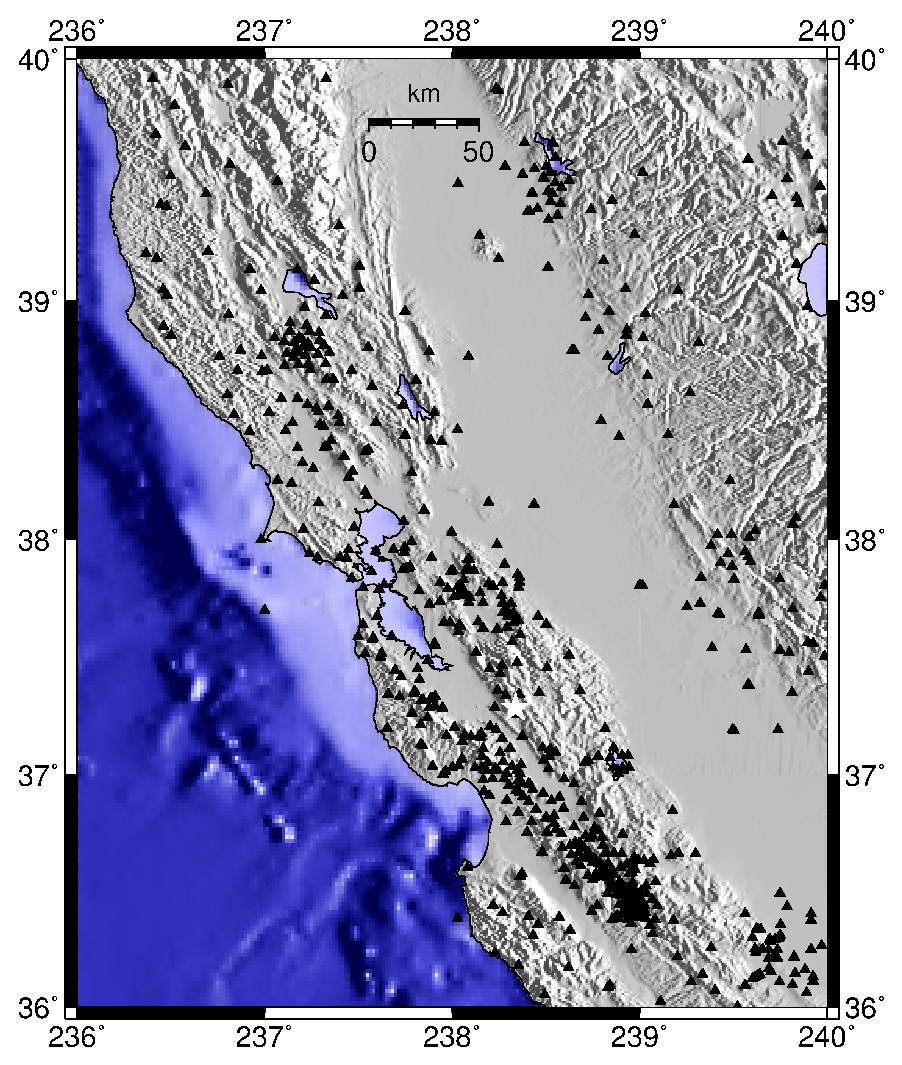
\includegraphics[width = 20pc]{diags/CalaverasMap/gmt_california/CaliforniaCalaverasMap1.eps}
\caption{Elevation in California showing location
of the 308 event Calaveras cluster (black star) and 805 seismic stations (red triangles).}
\label{fig:-eqopti-California-Calaveras}
\end{figure}


\begin{figure}
\includegraphics{diags/CalaverasLoc1.eps}
\caption{Comparison of earthquake hypocenters using three different methods: catalogue location (column 1), hypoDD with all
308 events (column 2) and CWI example 1 (column 3).
Note that in the case of the CWI locations we consider only the 68 earthquakes in red, the
blue events are shown for the purpose of orientation only.}
\label{fig-69Calaverasevents_eg1}
\end{figure}


\begin{figure}
\noindent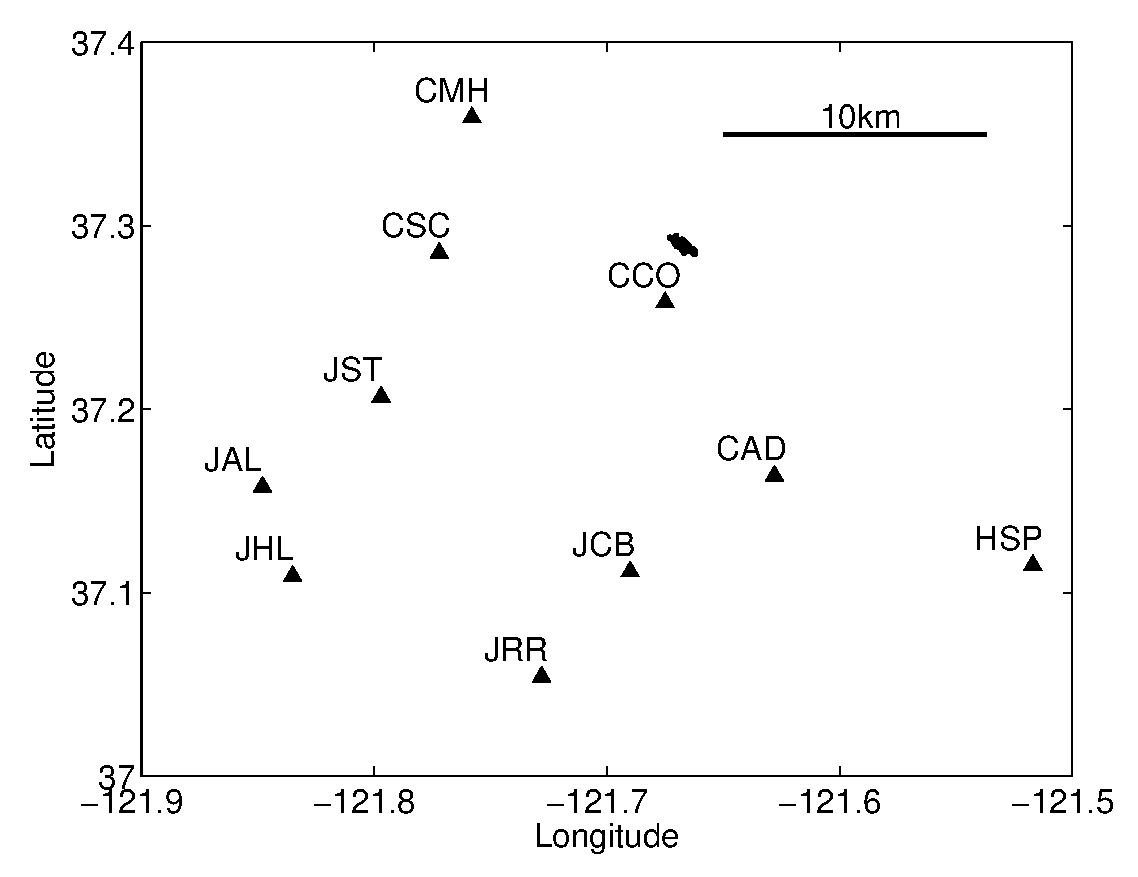
\includegraphics[width = 20pc]{diags/CalaverasMap/matlab/Calaveras_substationmap}
\caption{Location of the 10 stations (red triangles) used to relocate the Calaveras events.
Stations are removed one at a time according to the order in Table \ref{tab:Calaveras-stationremoval} and the events
relocated (see Figures \ref{fig-68Calaveras_CWIxyloc-statremove} to \ref{fig-68Calaveras_hypoDDyzloc-statremove}).
The 304 Calaveras events are indicated with black circles.}
\label{fig:-eqopti-Calaveras-substations}
\end{figure}

\begin{figure}
\includegraphics[angle=90,height = 50pc]{diags/CalaverasLoc2.eps}
\caption{....}
\label{fig-CWIreducesstats}
\end{figure}


\begin{figure}
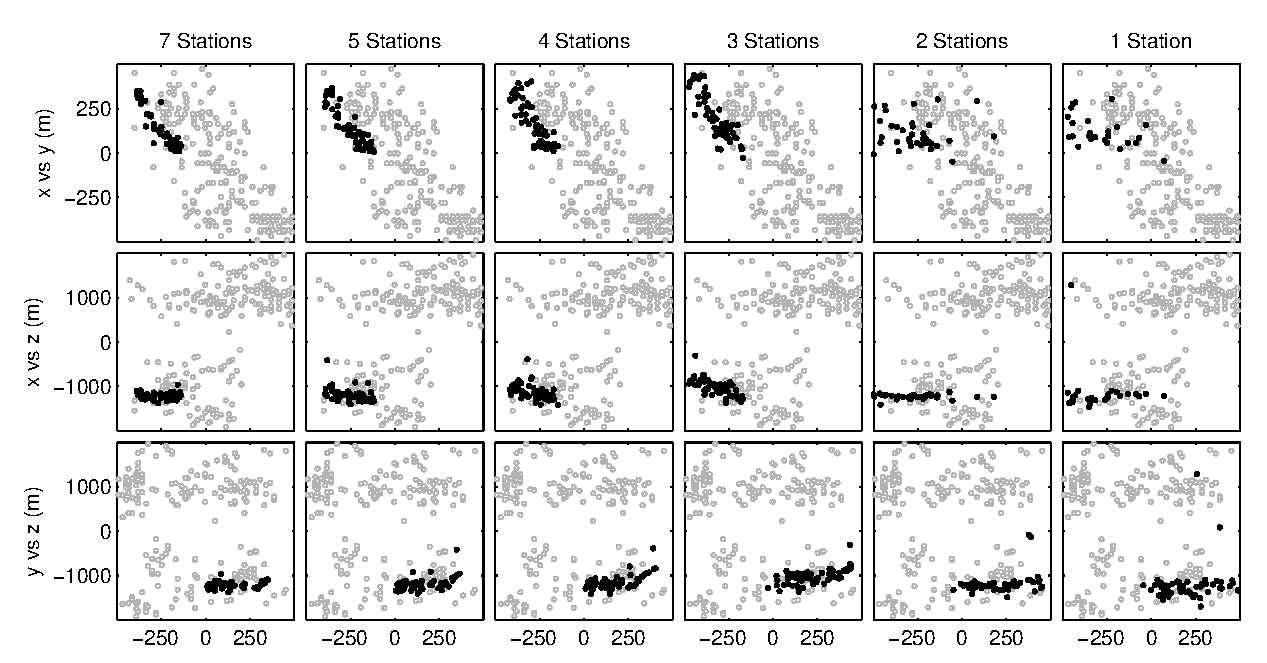
\includegraphics[angle=90,height = 50pc]{diags/CalaverasLoc3.eps}
\caption{....}
\label{fig-HYPODDreducesstats}
\end{figure}



\begin{figure}
\noindent\includegraphics[width = 20pc]{diags/CalaverasLoc4.eps}
\caption{Statistics on coordinate differences for reduced station inversions. Differences
are computed between the inversion results (CWI and hypoDD) and the complete hypoDD
locations for all 308 events. The top subplot illustrates the number of constrainable
events in the CWI and hypoDD inversions as a function of the stations considered.}
\label{fig-statremoval_summarystats}
\end{figure}


\begin{figure}
\noindent\includegraphics{diags/CalaverasLoc5.eps}
\caption{Locations of the 68 Calaveras earthquakes combining all available coda wave and travel time constraints with three different
levels of uncertainty on the travel time PDFs. Column 1 sets $\sigma_x = \sigma_y = 19.5$\,m and $\sigma_z = 15$\,m
(after \citealp{dr_Waldhauser08a}), Column 2 uses $\sigma_x = \sigma_y = 3 \times19.5$\,m and $\sigma_z = 3\times15$\,m and
column 3 considers $\sigma_x = \sigma_y = 152$\,m and $\sigma_z = 232$\,m (after \citealp{dr_Shearer97a}). }
\label{fig-68Calaverasevents_ttandcoda1}
\end{figure}

\begin{figure}
\noindent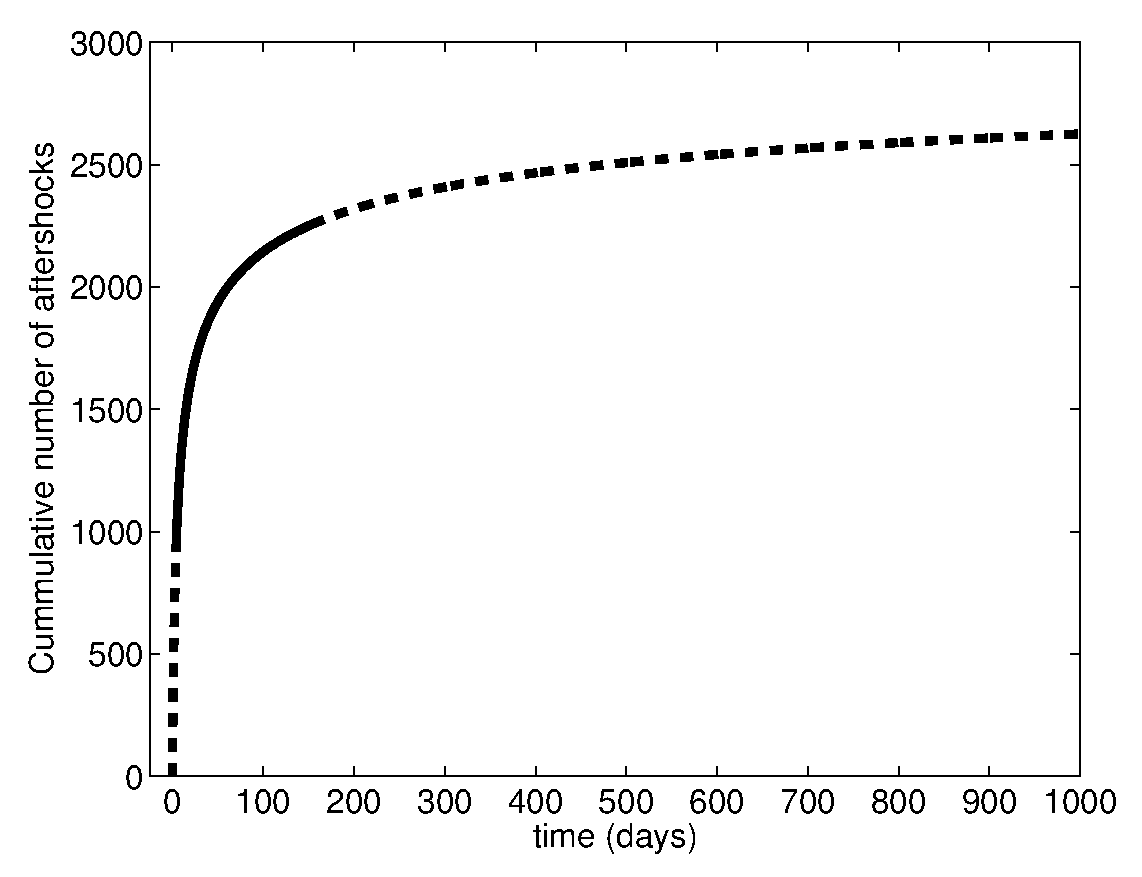
\includegraphics[width = 20pc]{diags/OmoriFigure.eps}
\caption{Cumulative number of aftershocks for the Hokkaido-Nansei-Oki, Japan
$M_s=7.8$ earthquake of 12 July 1993 according to the best fitting modified Omori Formula
\citep{dr_Utsu95a}. The leftmost dashed, middle solid and rightmost dashed signify aftershocks occurring before, during and
after the deployment of a temporary array installed 7 days after the main shock and left for
65 days.}
\label{fig:Omorifigure}
\end{figure}

\begin{figure}
\noindent\includegraphics{diags/CalaverasLoc6.eps}
\caption{Left - Combined travel time and coda wave inversions using travel time constraints on
22 (or 32\%) of the events and coda waves from station CCO only. All travel time based uncertainties
are assigned $\sigma_x = \sigma_y = 3 \times19.5$\,m and $\sigma_z = 3\times15$\,m. Right - travel time
relocation only (i.e. no CWI) using ........}
\label{fig-68Calaverasevents_ttsubsetandcoda1}
\end{figure}

\clearpage
\begin{table}
\caption{Stations considered when exploring the effect of reduced station coverage.}
\label{tab:Calaveras-stationremoval}
\begin{tabular}{|r|l|}
\hline
Number of & Station Names\\
Stations  & \\
\hline
10 & CCO, JCB, JST, CMH, HSP, JAL, CSC, JST, CAD, JHL, JRR\\
9  & CCO, JCB, JST, CMH, HSP, JAL, CSC, JST, CAD, JHL\\
8  & CCO, JCB, JST, CMH, HSP, JAL, CSC, JST, CAD\\
7  & CCO, JCB, JST, CMH, HSP, JAL, CSC \\
6  & CCO, JCB, JST, CMH, HSP, JAL \\
5  & CCO, JCB, JST, CMH, HSP \\
4  & CCO, JCB, JST, CMH \\
3  & CCO, JCB, JST \\
2  & CCO, JCB \\
1  & CCO \\
\hline
\end{tabular}
\end{table}

\end{document}

%%%%%%%%%%%%%%%%%%%%%%%%%%%%%%%%%%%%%%%%%%%%%%%%%%%%%%%%%%%%%%%

More Information and Advice:

%  SECTION HEADS

 ---------------
 Level 1 head

 Use the \section{} command to identify level 1 heads;
 type the appropriate head wording between the curly
 brackets, as shown below.

 Capitalize the first letter of each word (expect for
 prepositions, conjunctions, and articles that are
 three or fewer letters).

 Do not hyphenate level 1 heads. To break lines,
 type \protect\\ where you want the break to occur.
 AGU prefers the inverted triangle, breaking before
 prepositions, conjunctions, and articles, if possible.

An example:
\section{Level 1 Head: Introduction}

 ---------------
 Level 2 head

 Use the \subsection{} command to identify level 2 heads.

 Capitalize the first letter of each word (expect for
 prepositions, conjunctions, and articles that are
 three or fewer letters).

 Do not hyphenate level 1 heads. To break lines,
 type \protect\\ where you want the break to occur.
 AGU prefers the inverted triangle, breaking before
 prepositions, conjunctions, and articles, if possible.

\subsection{Level 2 Head} An example.

 ---------------
 Level 3 head

 Use the \subsubsection{} command to identify level 3 heads

 Capitalize only the first letter of the first word, acronyms,
 first letter of proper nouns, and first letter of first word
 after a colon.

 Hyphenation is permitted in level 3 heads, if needed.

\subsubsection{Level 3 Head} An example.

\subsubsubsection{Level 4 Head} An example.

%% ------------------------------------------------------------------------ %%
%
%  IN-TEXT LISTS
%
%% ------------------------------------------------------------------------ %%

% Do not use bulleted lists; enumerated lists are okay.
 \begin{enumerate}
 \item
 \item
 \item
 \end{enumerate}

%% ------------------------------------------------------------------------ %%
%
%  EQUATIONS
%
%% ------------------------------------------------------------------------ %%

% Single-line equations are centered.

 Math coded inside display math mode \[ ...\]
 will not be numbered e.g.:
 \[ x^2=y^2 + z^2\]

 Math coded inside \begin{equation} and \end{equation} will
 be automatically numbered e.g.:
 \begin{equation}
 x^2=y^2 + z^2
 \end{equation}

% IF YOU HAVE MULTI-LINE EQUATIONS, PLEASE
% BREAK THE EQUATIONS INTO TWO OR MORE LINES
% OF SINGLE COLUMN WIDTH (20 pc, 8.3 cm)
% using double backslashes (\\).

% To create multiline equations, use the
% \begin{eqnarray} and \end{eqnarray} environment
% as demonstrated below.
\begin{eqnarray}
  x_{1} & = & (x - x_{0}) \cos \Theta \nonumber \\
        && + (y - y_{0}) \sin \Theta  \nonumber \\
  y_{1} & = & -(x - x_{0}) \sin \Theta \nonumber \\
        && + (y - y_{0}) \cos \Theta.
\end{eqnarray}

If you don't want an equation number, use the star form:
\begin{eqnarray*}...\end{eqnarray*}

% Break each line at a sign of operation
% (+, -, etc.) if possible, with the sign of operation
% on the new line.

% Indent second and subsequent lines to align with
% the first character following the equal sign on the
% first line.

% Use an \hspace{} command to insert horizontal space
% into your equation if necessary. Place an appropriate
% unit of measure between the curly braces, e.g.
% \hspace{1in}; you may have to experiment to achieve
% the correct amount of space.

% There is another multiline equation environment:
% \begin{aguleftmath}...\end{aguleftmath}
% The equation is aligned left and the second line indents to
% the width of a paragraph indent (AGU style)


%% ------------------------------------------------------------------------ %%
%
%  EQUATION NUMBERING: COUNTER
%
%% ------------------------------------------------------------------------ %%

% You may change equation numbering by resetting
% the equation counter or by explicitly numbering
% an equation.

% To explicitly number an equation, type \eqnum{}
% (with the desired number between the brackets)
% after the \begin{equation} or \begin{eqnarray}
% command.  The \eqnum{} command will affect only
% the equation it appears with; LaTeX will number
% any equations appearing later in the manuscript
% according to the equation counter.
%
% To reset the equation counter, place the setcounter{equation}
% command in front of your equation(s).
%\setcounter{equation}{0}

% Set the equation counter to 0 if the next
% number needed is 1 or set it to 7 if the
% next number needed is 8, etc.
%
% The \setcounter{equation} command does affect
% equations appearing later in the manuscript.

% If you have a multiline equation that needs only
% one equation number, use a \nonumber command in
% front of the double backslashes (\\) as shown in
% the multiline equation above.



%%%%%%%%%%%%%%%%%%%%%%%%%%%%%%%%%%%%%%%%%%%%%%%%%%%%%%
%% Landscape figure and table examples
%
% ---------------
% Landscape (broadside) figure/table
% (These objects will not display properly in draft mode, use galley.)
%
% ONE-COLUMN landscape figure and table
%
% \begin{landscapefigure}
% \includegraphics[height=.75\mycolumnwidth,width=42pc]{samplefigure.eps}
% \caption{Caption text here}
% \end{landscapefigure}
%
% \begin{landscapetable}
% \caption{Caption text here}
% \begin{tabular*}{\hsize}{@{\extracolsep{\fill}}lcccc}
% \tableline
% ....
% \tableline\\
% \multicolumn5l{(a) Algorithms from Numerical Recipes}\\
% \end{tabular*}
% \tablenotetext{}{}
% \tablecomments{}
% \end{landscapetable}
%
% FULL-PAGE landscape figures and tables
%
% \begin{figure*}[p]
% \begin{landscapefigure*}
% illustration here
% \caption{caption here}
% \end{landscapefigure*}
% \end{figure*}
%
% \begin{table}[p]
% \begin{landscapetable*}
% \caption{}
% \begin{tabular*}{\textheight}{@{\extracolsep{\fill}}lccrrrcrrr}
% ....
% \end{tabular*}
% \begin{tablenotes}
% ...
% \end{tablenotes}
% \end{landscapetable*}
% \end{table}
%
